\section{Introduction: a common problem behind local results}
The twin-prime problem asks for infinitely many prime pairs at the fixed displacement $2$. Producing an expression that resembles a correlation sum, or a finite matrix with a small norm, is not enough. If a method transfers the original counting problem to another space, its coefficients, support, quantifiers, and normalization must travel with it. Omitting any of these can produce a correct statement that does not apply to the original problem.

The research archive contains successive local investigations numbered TPC1--TPC418, together with prototypes, source-unavailable markers, and later unnumbered work. Its development was problem-driven: an obstruction motivated a different representation, and a source audit sometimes required the actual object to be identified again. A chronological condensation would preserve this history without necessarily preserving the mathematical dependencies. We instead use Figure~\ref{fig:map} as a shared coordinate system and reconstruct a readable argument, leaving material outside that argument in a traceable companion index.

\begin{figure}[p]
\centering
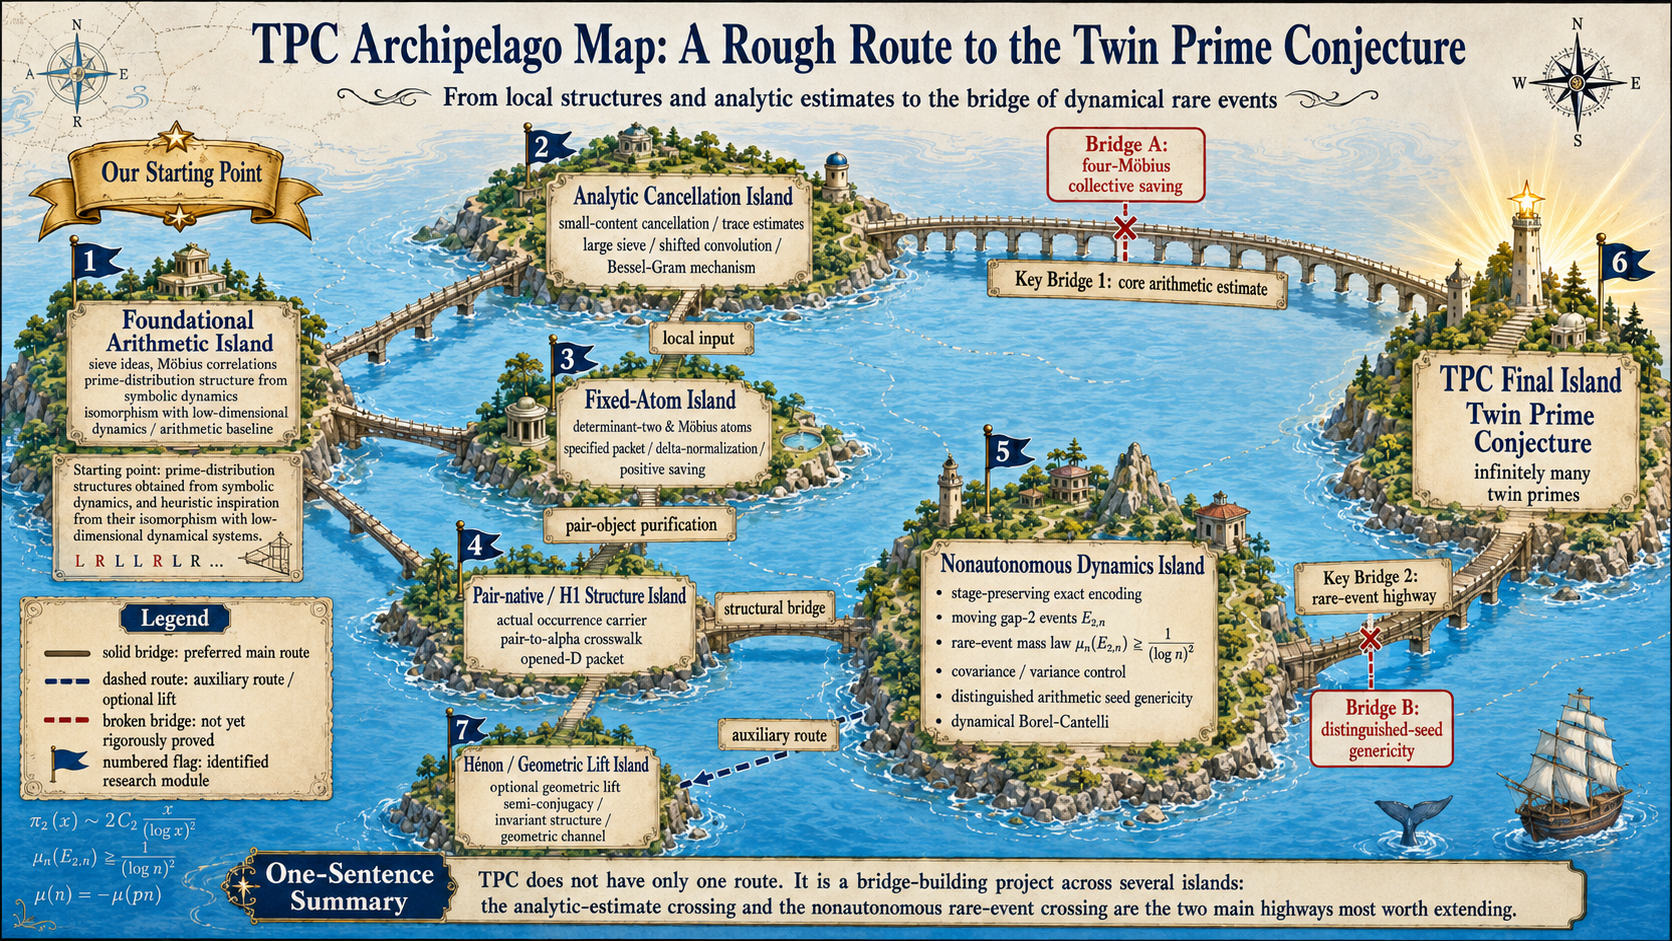
\includegraphics[width=\textwidth]{figures/tpc_route_en.png}
\caption{The user's English seven-island map, reproduced unchanged. Islands name objects and tasks, not completed steps. Solid and dashed connections depict proposed main and auxiliary routes; broken bridges indicate unproved transfers, not impossibility for every method. Schematic labels and formulae do not certify isomorphisms, positive savings, or twin-prime asymptotics: the hypotheses and qualifications in the text govern all mathematical claims. In particular, rare-event mass does not establish recurrence at the arithmetic seed. Map Bridge A contains both archive Gate A and Gate B; map Bridge B is the distinguished-seed dynamical bridge, not a filename containing ``Bridge-B.'' Enlarge the image for small labels; an identical full-resolution companion is supplied.}
\label{fig:map}
\end{figure}

\subsection{One framework, two substantive gaps}
The analytic route seeks to pass from local correlation structure to signed collective cancellation with the complete coefficients. One target considered here has natural scale $xQ^2$. To be an effective input to the specified endpoint interface, it must exhibit a power saving strictly exceeding $1/400$. Exact identities preserve the object but do not themselves supply that saving. Islands 3 and 4 concern the identification of local atoms and actual occurrences; Island 2 concerns the required estimates.

The dynamical gap is different. Adequate event mass and covariance control in an encoding system do not show that the particular orbit selected by arithmetic belongs to the good set. A statement about almost every initial point need not hold at a prescribed one. Calling that point ``typical'' cannot remove the quantifier gap. A geometric lift that merely changes the representation cannot supply the missing input either.

\subsection{Results retained in this synthesis}
The analytic exposition develops four groups of statements that can be checked separately:
\begin{enumerate}
\item An exact decomposition and row-energy bounds for the actual operator, under specified fixed-shift coefficients, unit masks, and kernel conventions, without substituting a model matrix.
\item A constant-vector norm lower bound, lower bounds for the actual coefficient norms, and a growing-dimensional obstruction to low-rank repairs. These restrict particular bounding methods, not the size of the actual mixed scalar.
\item An exact full-range Kloosterman representation and the norm of a one-short/one-complete array interface, separating algebraic representation, support compression, and signed reassembly.
\item An explicit partition with uniform derivative control and a paid collective boundary bound in the original mixed scalar, leaving the signed interior estimate open.
\end{enumerate}
The dynamical section additionally gives the $O(N)$ variance and Haar-almost-everywhere infinite-recurrence proof for the actual moving sieve events, separately from the unproved assertion at seed $0$. These are unified statements and reorganized proofs of archived results; no first-discovery or optimality claim is made. The appendix distinguishes the evidentiary roles of earlier finite certificates and later growing-model results, rather than counting them as savings for the actual arithmetic problem.

\subsection{Relation to existing mathematical inputs}
Our prime-counting input is the classical prime number theorem and its partial-summation consequences~\cite{selberg1949}. The second-moment estimate for the hybrid coefficient uses the unconditional Mertens product baseline, stated at the beginning of~\cite{lamzouri2015}; none of that paper's conditional conclusions on bias distributions is used. Frequency separation, positive-semidefinite compression, finite Fourier orthogonality, and spectral min--max arguments are standard tools in the structural proofs, not new prime-pair theorems.

The critical-interval bilinear estimate of Blomer--Pascadi~\cite{blomer2026} supplies an external benchmark: with the appropriate lengths and coprimality conditions, a Kloosterman bilinear form admits a local power saving. We use only the square-root-length specialization of their Theorem~1.1 and examine whether the actual representation satisfies its input conditions. The existence of that theorem is not an estimate for the complete arithmetic expression.

This article is not an exhaustive literature survey, and the number of internal documents is not a substitute for comparison with external work. It is a mathematical synthesis draft for a delimited research program. Submission would still require contribution positioning, a fuller bibliography, verification of all selected historical dependencies, and independent mathematical scrutiny of the complete argument.

\subsection{Reading guide}
Section~\ref{sec:arithmetic} fixes the endpoint and the transfer requirements. Section~\ref{sec:structure} treats the fixed atom and occurrence interfaces. Sections~\ref{sec:operator}--\ref{sec:boundary} develop the analytic core on one common object. Section~\ref{sec:dynamics} separates metric recurrence, the distinguished seed, and geometric attachment. Section~\ref{sec:bridges} assembles the two conditional bridge ledgers. The appendices distinguish model evidence and document provenance.
Readers need not read every historical manuscript in sequence to understand the main text; exact sources, material not selected for this synthesis, and the scope of review can be found in the accompanying source matrix and full catalog.
